\chapter{Bayesian Decisions for Lawyers}
\label{ch:decisions}

\section{Four questions}

Any legal decision, from a magistrate's bail order to a Supreme Court judgment, can be analysed by asking four questions. What are the possible actions? What are the possible states of the world? What is the consequence of each action in each state, and how good or bad is it? And how probable is each state, given the evidence? Bayesian decision theory answers the last question with Bayes' rule and combines the answers to all four with a single principle: choose the action with the smallest expected loss\index{expected loss}. This chapter sets out the method step by step, connects it to the language of Type I and Type II errors that lawyers meet in statistics and forensic science, and works through examples. Later chapters assume it.\index{decision theory}

\section{Objectives}

A decision needs an objective. In law, objectives are set by legislation, by precedent and by the purposes courts attribute to rules. The criminal law aims to punish and deter the guilty while protecting the innocent. Tort aims to compensate victims and to give actors incentives to take care. Contract aims to give effect to agreements and to make promises reliable. Procedure aims to resolve disputes accurately, quickly and at reasonable cost. Each objective implies a way of ranking outcomes, and the ranking is what decision theory calls a utility or, with the sign reversed, a loss.\index{objectives}

Two features of legal objectives matter for what follows. First, they are plural: a court wants accuracy, speed, low cost, fairness and legitimacy, and these conflict. A decision rule must trade them off, and the trade off should be stated. Second, they belong to society, not to the analyst. Decision theory does not tell a legislature how much worse a false conviction is than a false acquittal. It tells the legislature what its rules imply about that ratio, and what rules would implement any ratio it chooses.

\section{Actions, states and losses}

Let $\mathcal{A}$ be the set of actions open to the decision maker and $\Theta$ the set of states of the world. A loss function\index{loss function} $L(a,\theta)$ gives the loss from action $a$ when the state is $\theta$. For a criminal trial the simplest version has two actions, convict and acquit, two states, guilty and innocent, and a two by two table of losses (Table~\ref{tab:loss}). Correct decisions have zero loss; the two errors have losses $c_I$ and $c_{II}$. In the notation of Chapter~\ref{ch:why}, with $c$ for convict, $a$ for acquit, $G$ for guilt and $\bar G$ for not $G$, $c_I = L(c,\bar G)$ and $c_{II} = L(a,G)$; elsewhere in this chapter $a$ is a generic action.

\begin{table}[ht]
\centering\small
\begin{tabular}{lcc}
\toprule
& Innocent & Guilty\\
\midrule
Acquit & $0$ & $c_{II}$ (false acquittal)\\
Convict & $c_{I}$ (false conviction) & $0$\\
\bottomrule
\end{tabular}
\caption{The loss table for a criminal verdict.}
\label{tab:loss}
\end{table}

The loss table is the place where values enter. It is not a technicality. Whoever sets the criminal standard of proof, a constitutional court, the common law or a legislature, is choosing $c_I/c_{II}$, whether it says so or not.

\section{Type I and Type II errors}

\subsection{The classical vocabulary}

Classical hypothesis testing distinguishes two errors. A Type I error rejects a true null hypothesis; a Type II error fails to reject a false one. In criminal law the null hypothesis is innocence. A Type I error is convicting an innocent person; a Type II error is acquitting a guilty one. The Type I error rate, $\alpha$, is the probability of convicting given innocence; the power, $1-\beta$, is the probability of convicting given guilt, so $\beta$ is the Type II error rate.\index{Type I error}\index{Type II error}

\subsection{The trade off}

For given evidence, the two error rates trade off. A stricter standard of proof reduces $\alpha$ and raises $\beta$; a laxer one does the reverse. The receiver operating characteristic, or ROC curve, plots power against $\alpha$ as the threshold varies (Figure~\ref{fig:roc}). Better evidence moves the whole curve up and to the left, reducing both errors at once. Choosing a threshold is choosing a point on the curve; improving procedure, by better forensic science, better investigation or better presentation, is moving the curve.\index{ROC curve}

\begin{figure}[t]
\centering
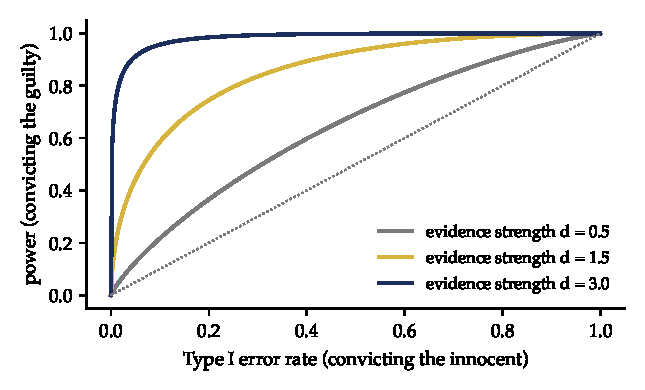
\includegraphics[width=\linewidth]{fig_roc}
\caption{ROC curves for evidence of three strengths. The standard of proof selects a point on a curve; better evidence moves the curve toward the top left corner, where both errors are small.}
\label{fig:roc}
\end{figure}

\subsection{From error rates to expected loss}

The classical approach fixes $\alpha$, conventionally at five per cent, and maximises power. The Bayesian approach minimises expected loss. If the prior probability of guilt in the cases that come to trial is $\pi$, the expected loss of a decision rule with error rates $\alpha$ and $\beta$ is
\begin{equation}
R = (1-\pi)\,\alpha\, c_I + \pi\,\beta\, c_{II}.
\label{eq:bayesrisk}
\end{equation}
Minimising $R$ over the rules on the ROC curve gives the point where the slope of the curve equals $(1-\pi)c_I/(\pi c_{II})$. The optimal $\alpha$ is not fixed at five per cent; it depends on the base rate and on the ratio of losses. In a population of defendants most of whom are guilty, a given threshold produces few false convictions in total; in a population most of whom are innocent, the same threshold produces many. This is why the Bayesian approach, which conditions on the evidence in each case, suits courts: it compares the posterior with a threshold set by the losses, and the base rate enters through the prior.\index{Bayes risk}

\subsection{Case by case: the posterior rule}

For an individual case, minimising expected loss gives the rule \eqref{eq:threshold} of Chapter~\ref{ch:why}, with $c_I = L(c,\bar G)$ and $c_{II} = L(a,G)$: convict if and only if
\begin{equation}
\Prob(\text{guilty}\given E) > \frac{c_I}{c_I + c_{II}} .
\end{equation}
This rule, applied case by case, also minimises the aggregate risk \eqref{eq:bayesrisk} across cases, provided the posteriors are computed with the same base rate and are calibrated. The two perspectives, the system's error rates and the individual posterior, are consistent: the posterior rule is the best way to run the system.

\begin{keybox}
Error rates and posteriors. A forensic test has a false positive rate of one per cent, used here as its Type I error rate, and power of ninety per cent. Of defendants tested, twenty per cent are guilty. Among positive results, the proportion from guilty defendants is $0.2\times 0.9/(0.2\times 0.9 + 0.8\times 0.01) = 0.957$. The test's error rate is one per cent, but about one positive in twenty three comes from an innocent person. If only two per cent of those tested were guilty, the proportion would fall to about $0.65$, and more than a third of positives would be innocent.
\end{keybox}

\section{Beyond two actions}

Real decisions have more than two actions. A sentencing judge chooses among discharge, fine, community order and custody of various lengths. A civil court chooses damages along a continuum. A regulator chooses among warning, fine and prosecution. Decision theory handles these by extending the loss table to each action and state, and by computing the expected loss of each action under the posterior.

\subsection{Continuous decisions and damages}

When the action is a number, such as an award of damages, and the state is the true loss $\theta$, a natural loss function is the squared error $(a-\theta)^2$ or the absolute error $|a-\theta|$. Under squared error the optimal award is the posterior mean of $\theta$; under absolute error it is the posterior median. If under compensation is worse than over compensation, an asymmetric absolute error loss leads to an award above the median, at a posterior quantile determined by the ratio of the losses. Chapter~\ref{ch:damages} develops this for the assessment of damages.\index{damages!as decision}

\subsection{Sequential decisions}

Some decisions come in sequences: whether to investigate, whether to charge, whether to accept a plea, whether to appeal. Each decision changes the information available for the next. Dynamic programming solves such problems backwards: the value of an early decision is the expected value of acting optimally afterwards. The value of information calculation of Chapter~\ref{ch:standards} is the simplest case: whether to gather more evidence before deciding.

\section{Costs of deciding}

Decisions have costs as well as consequences. A trial consumes judicial time, lawyers' fees, witnesses' time and the parties' attention. A complete objective adds the cost of the process to the expected loss of errors:
\begin{equation}
\text{total cost} = \text{cost of process} + \E[\text{loss from errors}].
\end{equation}
Spending more on a case usually reduces the expected loss from errors, by producing more and better evidence, but at a rising cost. The optimal investment equates the marginal cost of process with the marginal reduction in expected error cost. Louis Kaplow analysed this trade off in a classic article on the value of accuracy in adjudication \citep{kaplow1994}. Chapter~\ref{ch:systemcosts} applies it to the allocation of judges' time across a court system.\index{accuracy, value of}

\section{Objectives revisited: deterrence and incentives}

The losses in Table~\ref{tab:loss} describe the harm from errors in a single case. But legal decisions also shape behaviour. A rule that convicts too readily deters some innocent conduct; a rule that acquits too readily fails to deter crime. False convictions reduce deterrence, as Chapter~\ref{ch:becker} will show, because they impose sanctions whether or not one offends. The ex post loss from an error, what it costs the people in this case, and the ex ante effect of the rule on everyone's behaviour, can point in different directions. A full analysis includes both. In tort, for example, the ex post objective is to compensate the claimant accurately; the ex ante objective is to give defendants the right incentives to take care. Proportional liability for lost chances, taken up in Chapter~\ref{ch:tort}, is attractive partly because it serves both.

\section{A worked example: bail}

A magistrate must decide whether to release a defendant before trial. The actions are release and detain. The states are whether the defendant would, if released, fail to appear or commit an offence. Let the probability of such failure, given the risk assessment and the facts, be $r$. The loss from releasing a defendant who then fails is $H$, the harm to victims and the cost of recapture. The loss from detaining a defendant who would not have failed is $D$, the cost of detention to the defendant, the defendant's family and the state, which is proportional to the expected time to trial (taken here as twelve months). Release is optimal if $rH < (1-r)D$, that is if
\begin{equation}
r < \frac{D}{H + D}.
\end{equation}
If detention for the expected period costs one third as much as a failure, the threshold is one quarter: release anyone whose risk is below twenty five per cent. If delay doubles the cost of detention, the threshold rises to forty per cent. The analysis shows why delay in trials, the subject of Chapter~\ref{ch:india}, should change bail practice, and why risk assessment tools must be calibrated: the decision turns on the probability $r$, and a tool that overstates it detains people who should be released.

\section{A worked example: whether to sue}

A claimant must decide whether to bring a claim. The probability of winning is $p$, the damages if successful are $J$, the cost of litigating is $C$, and, under the English costs rule, the loser pays the winner's costs, so the claimant who loses pays the defendant's costs $C_D$ as well. A winner does not recover everything it spent: costs assessed on the standard basis usually fall well short of actual spend. Let $f$ be the fraction recovered, so that the claimant who wins recovers $fC$ and the claimant who loses pays $fC_D$. The expected value of suing under the English rule is
\begin{equation}
p\,J - C - (1-p)\,f\,C_D + p\,f\,C.
\end{equation}
The costs rules differ across systems, so it is worth comparing the common ones with the same $p$ and the same stakes. Take a claimant with a forty per cent chance of winning a hundred thousand pounds, with costs of thirty thousand on each side ($C = C_D = 30{,}000$). The recovery fraction is an assumption, not a fact about any case: we take $f = 2/3$, the figure commonly put as the typical recovery on a standard basis assessment, and apply it to both sides.

\begin{enumerate}[label=(\alph*)]
\item American rule: each side bears its own costs whatever the outcome. The claimant nets $70{,}000$ on winning and loses $30{,}000$ on losing, and the expected value is $40{,}000 - 30{,}000 = 10{,}000$.
\item English rule: costs follow the event (CPR 44.2(2)(a)). The claimant nets $100{,}000 - 30{,}000 + 20{,}000 = 90{,}000$ on winning and loses $30{,}000 + 20{,}000 = 50{,}000$ on losing. The expected value is $40{,}000 - 30{,}000 - 12{,}000 + 8{,}000 = 6{,}000$.
\item Qualified one-way costs shifting, which applies to English personal injury claims since April 2013 (CPR 44.13 to 44.17): a losing claimant ordinarily does not pay the defendant's costs, while a winning claimant still recovers part of its own. The claimant nets $90{,}000$ on winning and loses $30{,}000$ on losing, and the expected value is $40{,}000 - 30{,}000 + 8{,}000 = 18{,}000$.
\end{enumerate}

The claimant should sue if the expected value exceeds zero, adjusted for risk aversion. All three are positive here, but the rules differ in how much risk they impose. The spread between the winning and losing outcomes is $100{,}000$ under the American rule, $140{,}000$ under the English rule and $120{,}000$ under one-way shifting. The English rule gives the lowest expected value and the widest spread, so a risk averse claimant is the most likely to decline to sue, or to accept a settlement below the expected value, under it. A pre-action settlement offer, a topic Chapter~\ref{ch:becker} takes up, offers a certain amount instead. The break-even probability of winning is $0.30$ under the American rule, $5/14 \approx 0.36$ under the English rule and $0.25$ under one-way shifting, so the last encourages weak claims most. The English figures depend on the assumed recovery fraction: if $f = 1$ the English rule has expected value $40{,}000 - 30{,}000 - 18{,}000 + 12{,}000 = 4{,}000$. Litigation funding, the subject of Chapter~\ref{ch:funding}, changes this calculation by transferring risk.

\section{Summary}

Bayesian decision theory asks four questions and gives one answer. The questions are about actions, states, losses and probabilities. The answer is to minimise expected loss. Type I and Type II errors are the two ways of being wrong in a binary decision; their rates trade off along an ROC curve, and the standard of proof chooses a point on it according to the ratio of losses. Better evidence moves the curve. Costs of process, incentives and sequences of decisions extend the framework without changing its logic. The rest of the book applies it.

\section*{Notes and Questions}
\addcontentsline{toc}{section}{Notes and Questions}
\begin{enumerate}[label=\arabic*.]
\item Write down a loss table for a civil claim with actions judgment for claimant and judgment for defendant. What ratio of losses does the balance of probabilities imply?
\item For an ROC curve in which the evidence is a score that is normal with mean $0$ for the innocent and mean $d = 1.5$ for the guilty, both with standard deviation one, find the threshold that minimises expected loss when $\pi = 0.6$ and $c_I/c_{II} = 10$. What are $\alpha$ and $\beta$ at that threshold?
\item In the keybox example, find the base rate of guilt at which half of positive tests come from innocent people.
\item Under absolute error loss the optimal award is the posterior median. If under compensation is twice as bad as over compensation, at what posterior quantile should damages be set?
\item In the bail example, how should the threshold change if the expected time to trial falls from twelve months to three?
\item Recompute the English and one-way shifting expected values in the whether-to-sue example with $f = 1/2$. Which rule encourages weak claims?
\end{enumerate}

\section*{Further reading}
Lindley's \emph{Making Decisions} \citep{lindley1985}; Smith's \emph{Bayesian Decision Analysis} \citep{smith2010}; Kaplow on the value of accuracy \citep{kaplow1994}.
